\documentclass[11pt,a4paper]{article}
\usepackage[utf8]{inputenc}
\usepackage{amsfonts}
\usepackage{pdfpages}
\usepackage{eurosym}
\usepackage{hyperref}
\hypersetup{
    colorlinks=true,
    linkcolor=black,
    filecolor=magenta,      
    urlcolor=cyan,
    pdftitle={Overleaf Example},
    pdfpagemode=FullScreen,
    }
\usepackage{algpseudocode}
\usepackage{algorithm}
\usepackage{letltxmacro}
\usepackage{microtype}
\usepackage[left=3cm,right=3cm,bottom=3.5cm]{geometry}
\usepackage{emptypage}
\usepackage{amsmath,amssymb,amsthm, latexsym}
\usepackage[english,italian]{babel}
\usepackage{url}
\usepackage{caption}
\captionsetup{tableposition=top,figureposition=bottom,font=small,format=hang,labelfont={sf,bf}}
\usepackage{graphicx}
\usepackage{tabularx}
\usepackage{listings}
\usepackage{hyphenat}
\usepackage{subfig}
\pagestyle{empty}
\newcommand\AlCentroPagina[1]{%
\AddToShipoutPicture*{\AtPageCenter{%
\makebox(0,0){\includegraphics%
[width =0.9\paperwidth]{#1}}}}}

\begin{document}
\newcommand{\horrule}[1]{\rule{\linewidth}{#1}}
\lstset{language=Java} 
\lstset{basicstyle=\footnotesize\ttfamily}
\author{Silvio Baratto}
\title{
\normalfont \normalsize 
\href{https://github.com/SilvioBaratto/KD-tree}{github.com/SilvioBaratto/KD-tree} \\ [25pt] % Your university, school and/or department name(s)
\horrule{0.5pt} \\[0.4cm] % Thin top horizontal rule
\huge Parallel k-d tree OpenMP \& OpenMPI\\ % The assignment title
\horrule{2pt} \\[0.5cm] % Thick bottom horizontal rule
}
\maketitle
\tableofcontents
\newpage
\section{Introduction}
In computer science, a k-d dimensional tree is a space-partitioning data structure for organizing points in a k-dimensional space. k-d trees are a useful data structure for several applications, such as searches involving a multidimensional search key (e.g. range searches and nearest neighbor searches) and creating point clouds. k-d trees are a special case of binary space partitioning trees. In this brief report is presented a parallel implementations of k-d tree which uses two standard frameworks for parallel programming, namely OpenMP (shared memory) and MPI (distributed memory).
\section{Algorithm}
The construction of the tree is done by:
\begin{center}
\begin{itemize}
\item Finding median / pivot by medians of the input file. Each section of constant lenght is sorted bt $std::nth\_element$ from the C++ standard library. \\
\item Recursively proceed on left and right portions on the left and right of the found median.  \\
\item Terminate when length of a portion is 0. \\
\item Return root node.
\end{itemize}
\end{center}
The time complexity of the divide and conquer algorithm is $O(nlog(n))$ since the partition process always picks the middle element as pivot. The median of the medias is found in linear time, $O(n)$.\\
Time complexity for partitioning n datapoints:
\begin{equation*}
T(n) = 2T(n / 2)+ \theta{(n)}
\end{equation*}
\subsection{Implementation}
The KD-Tree implementation was made with C++17 and written using C++ templates so is a generic programming algorithm working with both float, integers and double numbers. The purpose of this code was to be as simple as possible to use from the point of view of a user. The goal was to generate a k-d tree from a file choosen from a local directory of the user, containing points in two dimension. To do this, the constructors of all the three classes (mpi, omp, serial) creates a non ordered vector of knodes using as points the ones in the dataset, in this way it has been possible also to use the standard library functions provided from C++17. \\
The implemented algorithm doesn’t use a sorting algorithm, but it uses the function provided by the standard
library “$std::nth\_element()$”. This function is a partial sorting algorithm that rearranges elements in [first,
last) such that:
\begin{center}
\begin{itemize}
\item the element pointed at by nth (the median) is changed to whatever element would occur in that position if [first, last) were sorted. \\
\item All of the elements before this new nth element (the median) are less than or equal to the elements after the new nth element. With this function, it’s possible to omit the implementation of a sorting algorithm because it has the best “worst expected running time”, that is $O(N)$. 
\end{itemize}
\end{center}
\begin{algorithm}
\caption{makeTree}
\begin{algorithmic}[1]
\Function{makeTree}{begin, end, axis}
\If{end $\leq$ begin}\Comment{base case}
\State return $\textit{nullptr}$
\EndIf
\State median $\gets$ begin + (end - begin) / 2
\State \Call{nth\_element}{begin, med, axis, cmp$(axis)$}
\State myaxis $\gets$ round robin approach between 0 and 1
\State knode[med].left $\gets$ $\Call{makeTree}{$begin, med, myaxis$}$
\State knode[med].right $\gets$ $\Call{makeTree}{$med + 1, end, myaxis$}$
\State \Return \text{\&{knode[med]}}
\EndFunction
\end{algorithmic}
\end{algorithm}
\subsection{OpenMP}
OpenMP is one of the application programming interfaces that facilitates the employment of a shared memory paradigm for parallelization within a node. Below the algorithm used in the implementation
\begin{algorithm}
\caption{makeTree}
\begin{algorithmic}[1]
\Function{makeTree}{begin, end, axis}
\If{end $\leq$ begin}\Comment{base case}
\State return $\textit{nullptr}$
\EndIf
\State median $\gets$ begin + (end - begin) / 2
\State \Call{nth\_element}{begin, med, axis, cmp$(axis)$}
\State myaxis $\gets$ round robin approach between 0 and 1
\color{blue}
\State{\#pragma omp task}
\color{black}
\State knode[med].left $\gets$ $\Call{makeTree}{$begin, med, myaxis$}$
\color{blue}
\State{\#pragma omp task}
\color{black}
\State knode[med].right $\gets$ $\Call{makeTree}{$med + 1, end, myaxis$}$
\State \Return \text{\&{knode[med]}}
\EndFunction
\Statex
\Function{makeTreeParallel}{begin, end, axis}
\color{blue}
\State{\#pragma omp parallel}
\State{\#pragma omp single}
\color{black}
\State root * $\gets$ $\Call{makeTree}{$begin, end, axis$}$
\State \Return root
\EndFunction
\end{algorithmic}
\end{algorithm}
\subsection{OpenMPI}
\begin{algorithm}[H]
\caption{makeTreeParallel}
\begin{algorithmic}[1]
\Function{makeTreeParallel}{begin, end, axis, nprocs, depth, comm, next}
\If{end $\leq$ begin}\Comment{base case}
	\State return $\textit{nullptr}$
\EndIf
\State median $\gets$ begin + (end - begin) / 2
\State \Call{nth\_element}{begin, med, axis, cmp$(axis)$}
\State myaxis $\gets$ round robin approach between 0 and 1
\If{rank != 0}
	\If{$nprocs / 2 != 2^{depth}$}
		\State depth $\gets$ depth + 1
		\State knode[med].left $\gets$ $\Call{makeTreeParallel}{$begin, med, myaxis, myaxis, nprocs, depth, comm, next$}$
		\State next = next + 2
		\State knode[med].left $\gets$ $\Call{makeTree}{$med + 1, end, myaxis, nprocs, depth, comm, next$}$
\Else
	\If{rank == next}
		\State knode[med].left $\gets$ $\Call{makeTree}{$begin, med, index$}$
		\color{red}
		\State serializeLeft $\gets$ $\Call{serializeNode}{$knode[med].left$}$
		\color{black}
		\color{blue}
		\State MPI\_Send(serializeLeft, length, MPI\_CHAR, 0, left\_tag, comm)
		\color{black}
	\EndIf
	\State next $\gets$ nprocs - 1 ? next + 1 : 1
	\If{rank == next}
		\State knode[med].right $\gets$ $\Call{makeTree}{$med + 1, end, index$}$
		\color{black}
\color{red}
		\State serializeRight $\gets$ $\Call{serializeNode}{$knode[med].right$}$
		\color{black}
		\color{blue}
		\State MPI\_Send(serializeRight, length, MPI\_CHAR, 0, right\_tag, comm)
		\color{black}
	\EndIf
\EndIf
\ElsIf{rank == 0}
	\If{$nprocs / 2 != 2^{depth}$}
		\State depth $\gets$ depth + 1
		\State knode[med].left $\gets$ $\Call{makeTreeParallel}{$begin, med, index, nprocs, depth, comm, rank$}$
		\State next $\gets$ next + 2
		\State knode[med].right $\gets$ $\Call{makeTreeParallel}{$med + 1, end, index, nprocs, depth, comm, rank$}$
	\Else 
		\color{blue}
		\State MPI\_Probe(next, left\_tag, comm, \&status)
		\State MPI\_Get\_Count(\&status, MPI\_CHAR, \&count)
		\State MPI\_Recv(buffer\_left, count MPI\_CHAR, next, left\_tag, comm, \&status)
		\color{red}
		\State knode[med].left $\gets$ $\Call{deserialize}{$buffer\_left$}$
		\color{black}
		\State next $\gets$ nprocs - 1 ? next + 1 : 1
		\color{blue}
		\State MPI\_Probe(next, right\_tag, comm, \&status)
		\State MPI\_Get\_Count(\&status, MPI\_CHAR, \&count)
		\State MPI\_Recv(buffer\_right, count MPI\_CHAR, next, left\_tag, comm, \&status)
		\color{red}
		\State knode[med].left $\gets$ $\Call{deserialize}{$buffer\_right$}$
		\color{black}
	\EndIf
\EndIf
\State \Return \text{\&{knode[med]}}
\EndFunction
\end{algorithmic}
\end{algorithm}
The code to implement the OpenMPI is quite different from the OpenMP. The strategy has been to divide for each process a sub-tree and combined them in the main process. The process 0 merge all the sub-trees and construct the final one. When the the half of the number of process is equal to the power of 2 to depth each process works alone creating the sub-tree in a serial way and sending it to the master process with rank 0. To send and receive the messagges has been used a serialize and deserialize function that increase a lot the performance time and has been the main problem in this implementation. 
\section{Strong and weak scalability}
\subsection{Strong scalability}
The strong scalability explain the performance of the parallel algorithm with the number of processors that increase while the problem size remains constant. To study the strong scalability it has been used:
\begin{itemize}
\item $N = 100000000$ 
\item $p \in \{1, 2, 4, 8, 16, 24, 32, 48\}$ 
\end{itemize}
From the graph above it's possible to see an huge difference between OpenMPI and OpenMP. The main problem of the OpenMPI implementation is the serialization and deserialization part of the code.  
\begin{figure}[H]
    \centering
    \subfloat[\centering Comparison between different implementation]{{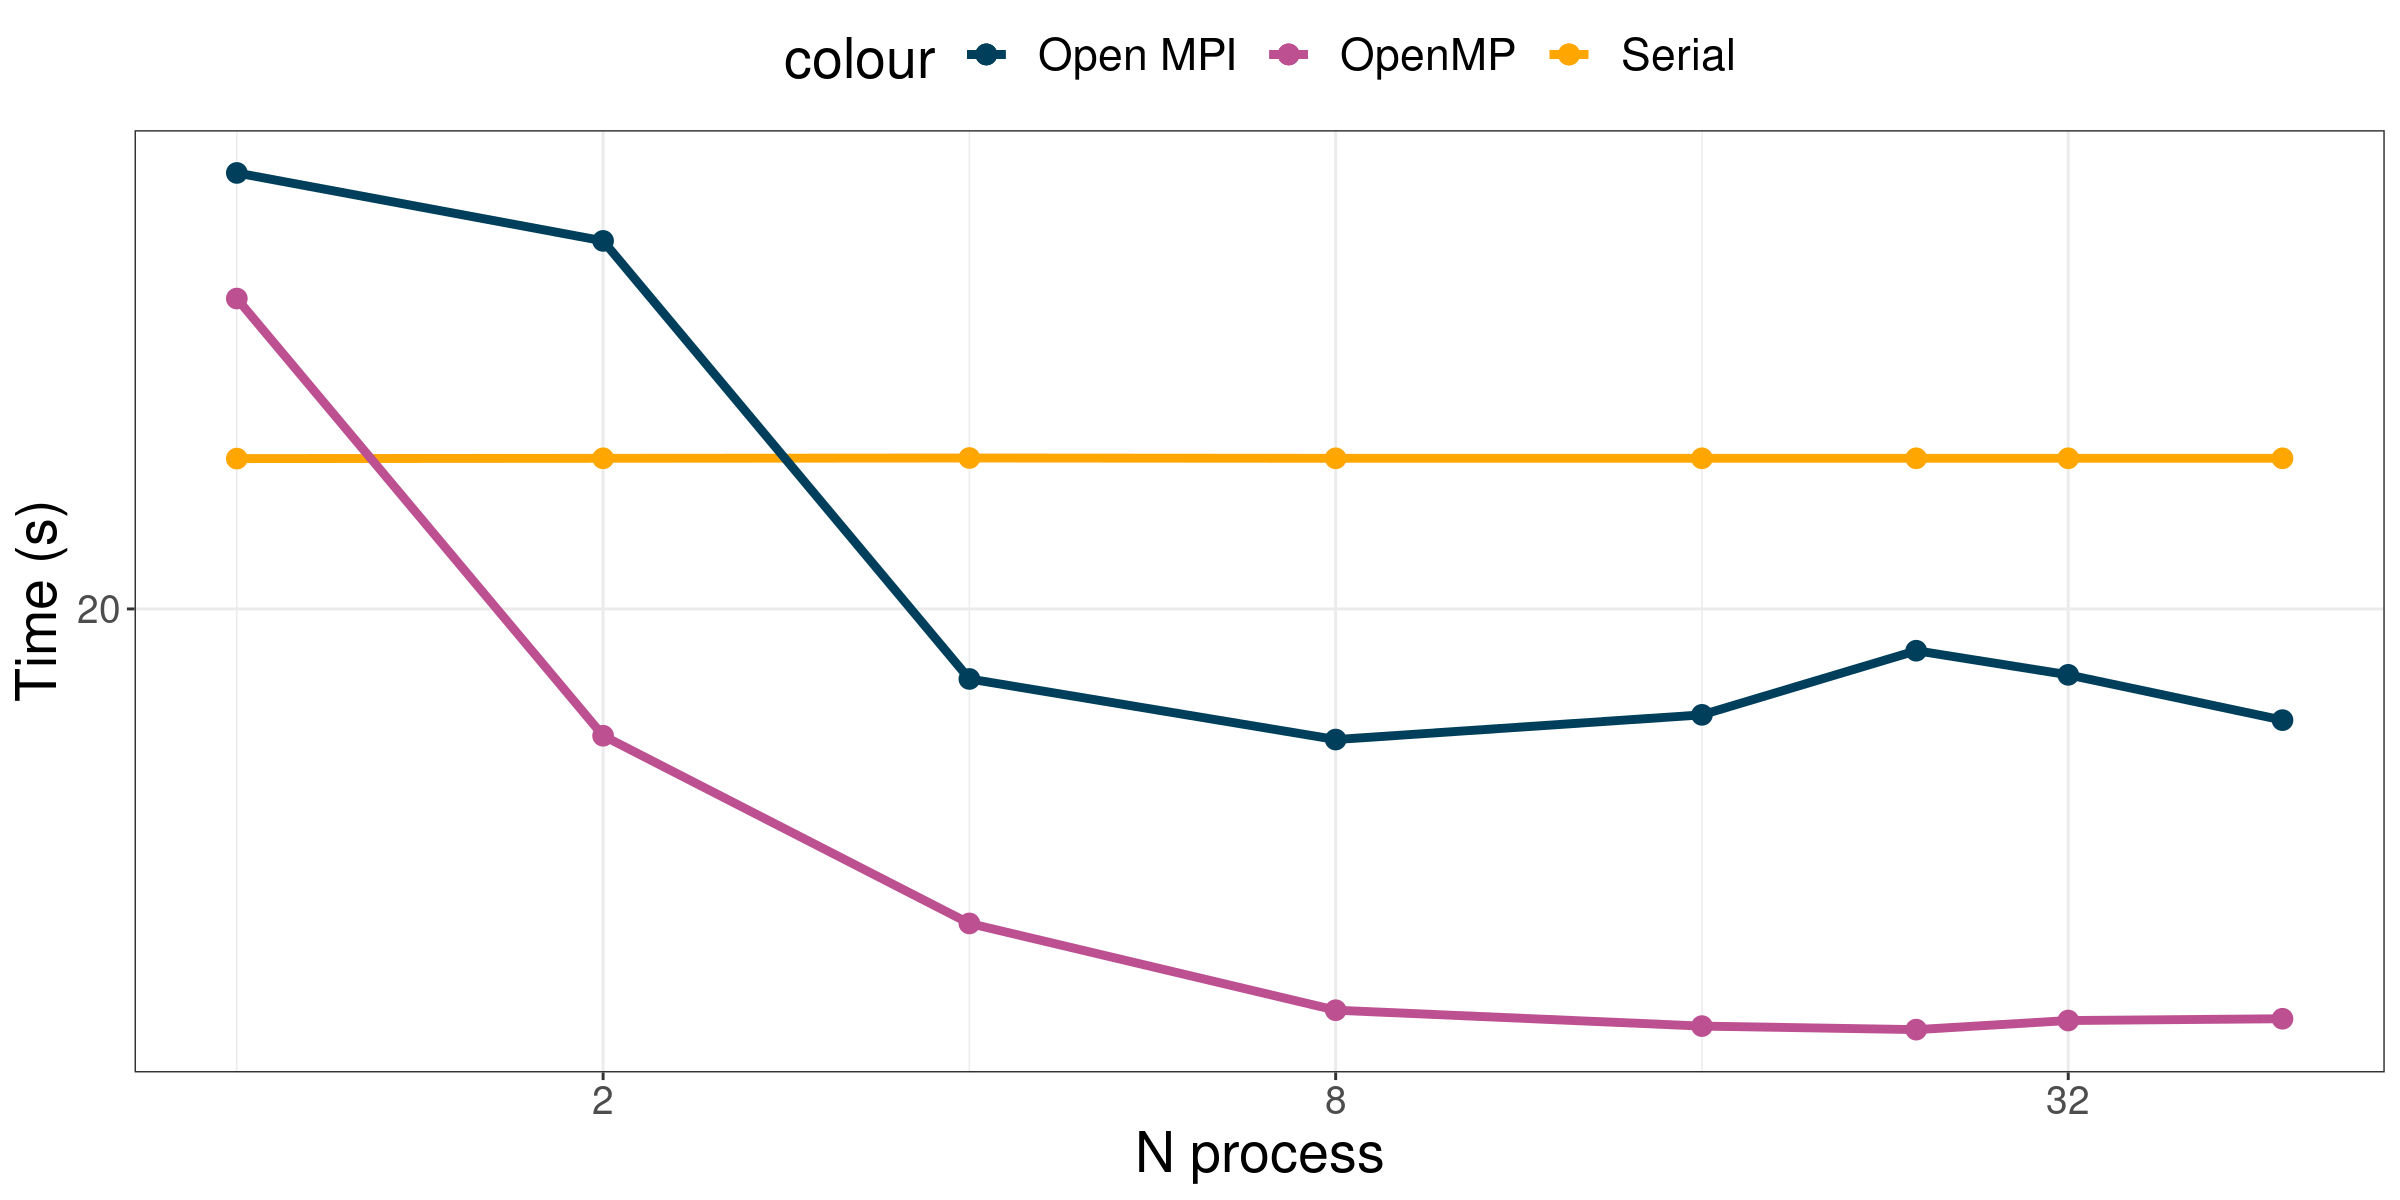
\includegraphics[width=15cm]{strong}}}
\end{figure}
The speedup is the ratio of the one-CPU execution time to the N-CPU parallel execution time: $S(P) = T(1)/T(P)$. When $S(P) = P$ it is considered a perfect speed-up. This in ”real-life” is not an ultimate goal, since the code usually has parts that need to execute in serial.  This happens because some parts of a program can’t be executed in parallel. This phenomenon is describes by the Amdahl’s Law, that is:
\begin{equation}
S(P) = \dfrac{1}{(1-P)/(P/N)}
\end{equation}
From the graph above OpenMP has best performance but Open MPI algorithm has greater margin for growth without serialization and deserialization.
\begin{figure}[H]
    \centering
    \subfloat[\centering Speedup OpenMP and OpenMPI]{{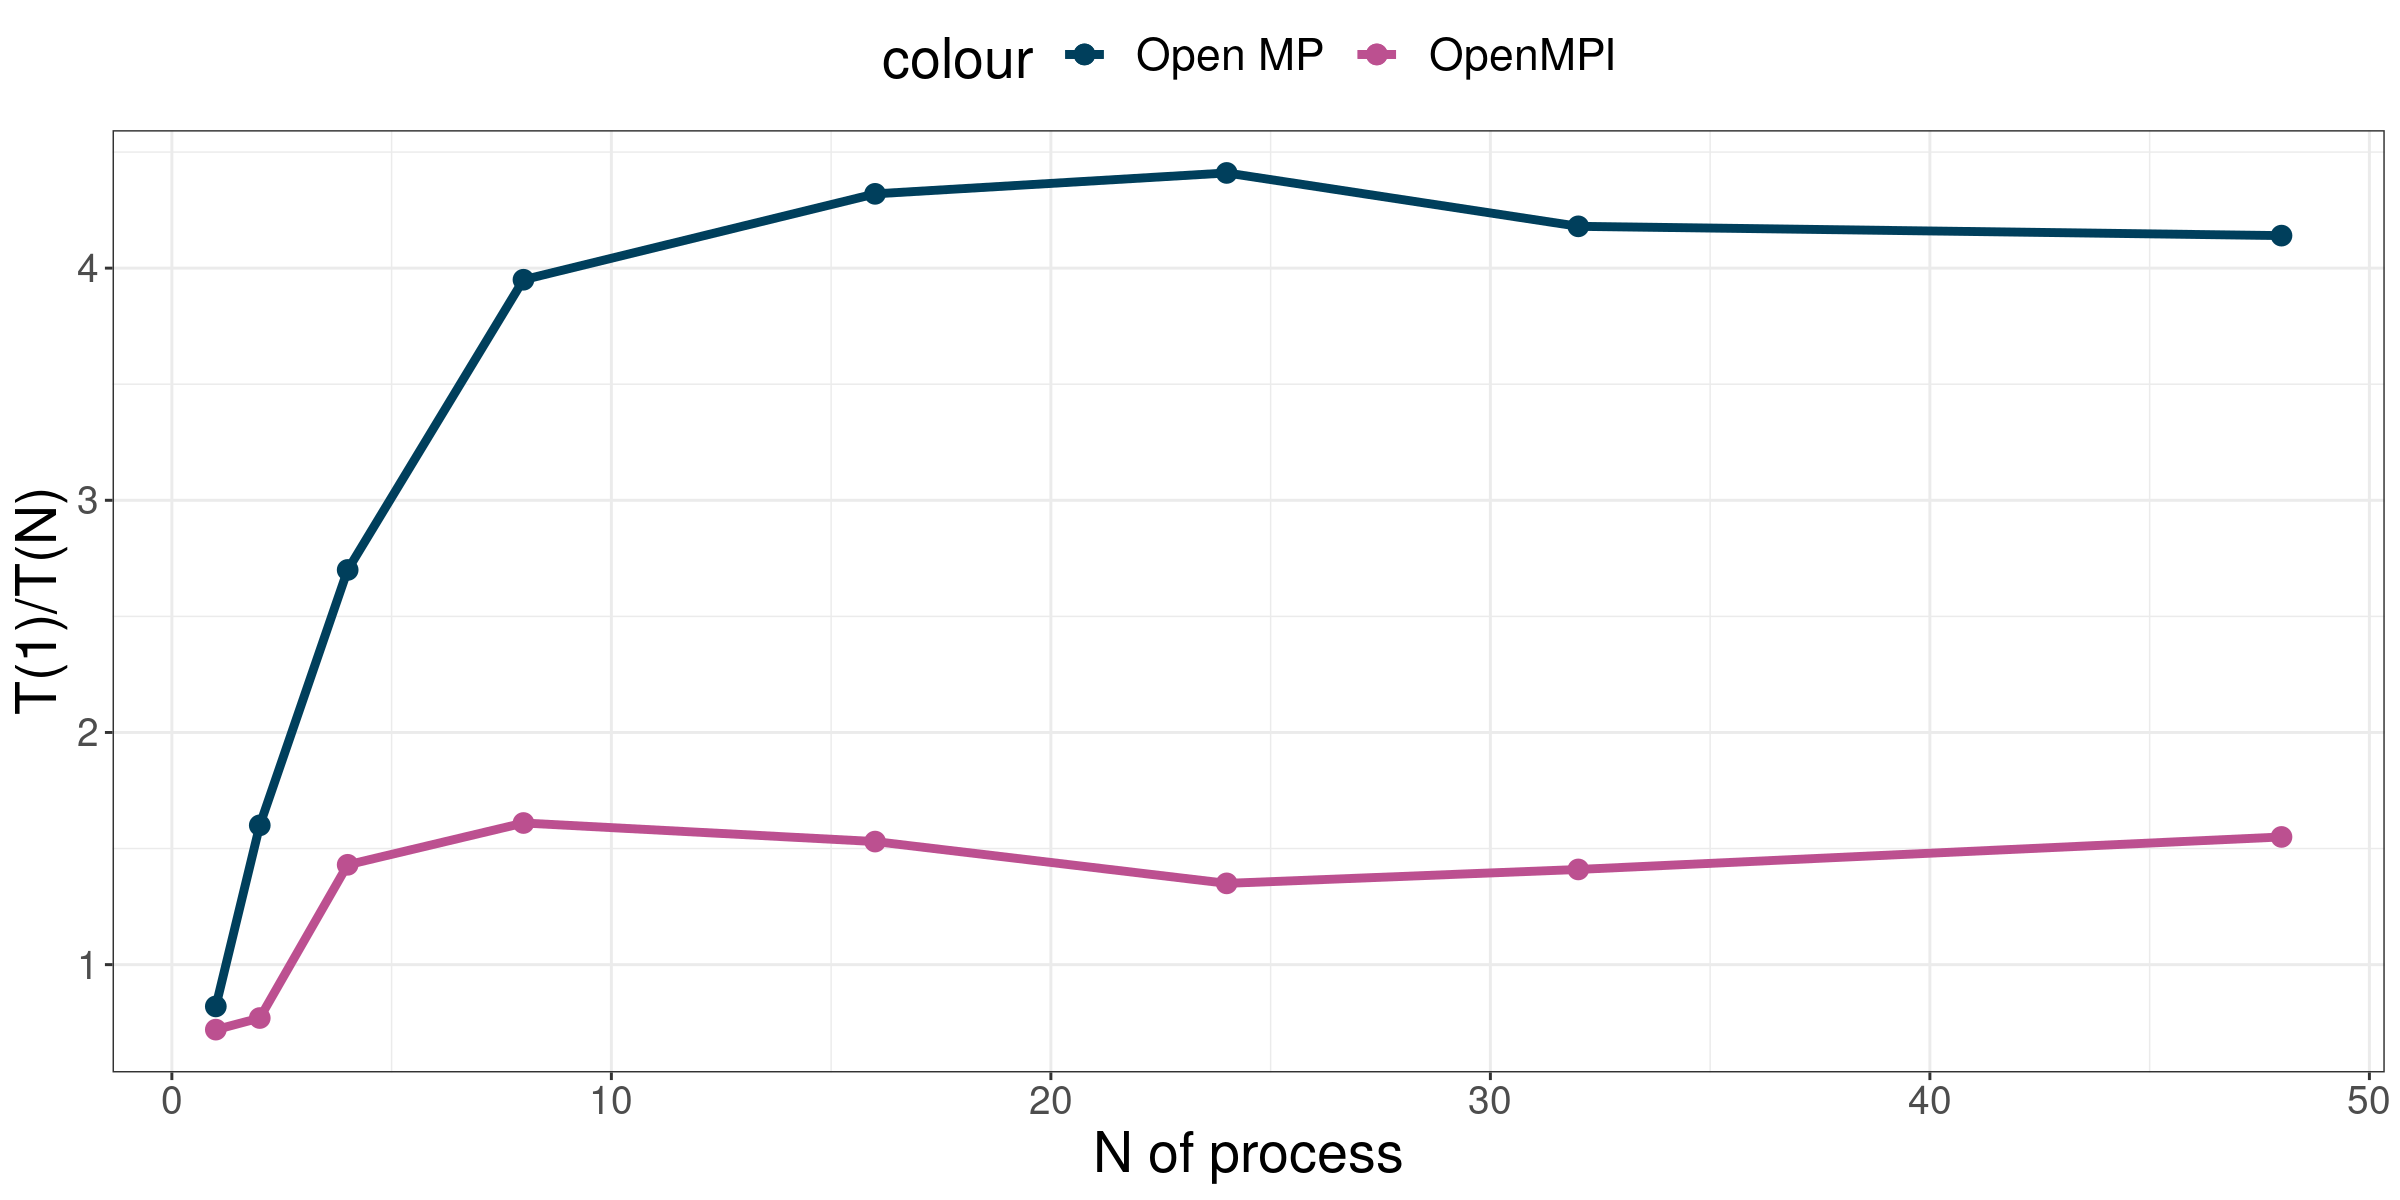
\includegraphics[width=15cm]{speedupStrong}}}
\end{figure} 
\begin{figure}[H]
    \centering
    \subfloat[\centering Strong scalability OpenMP]{{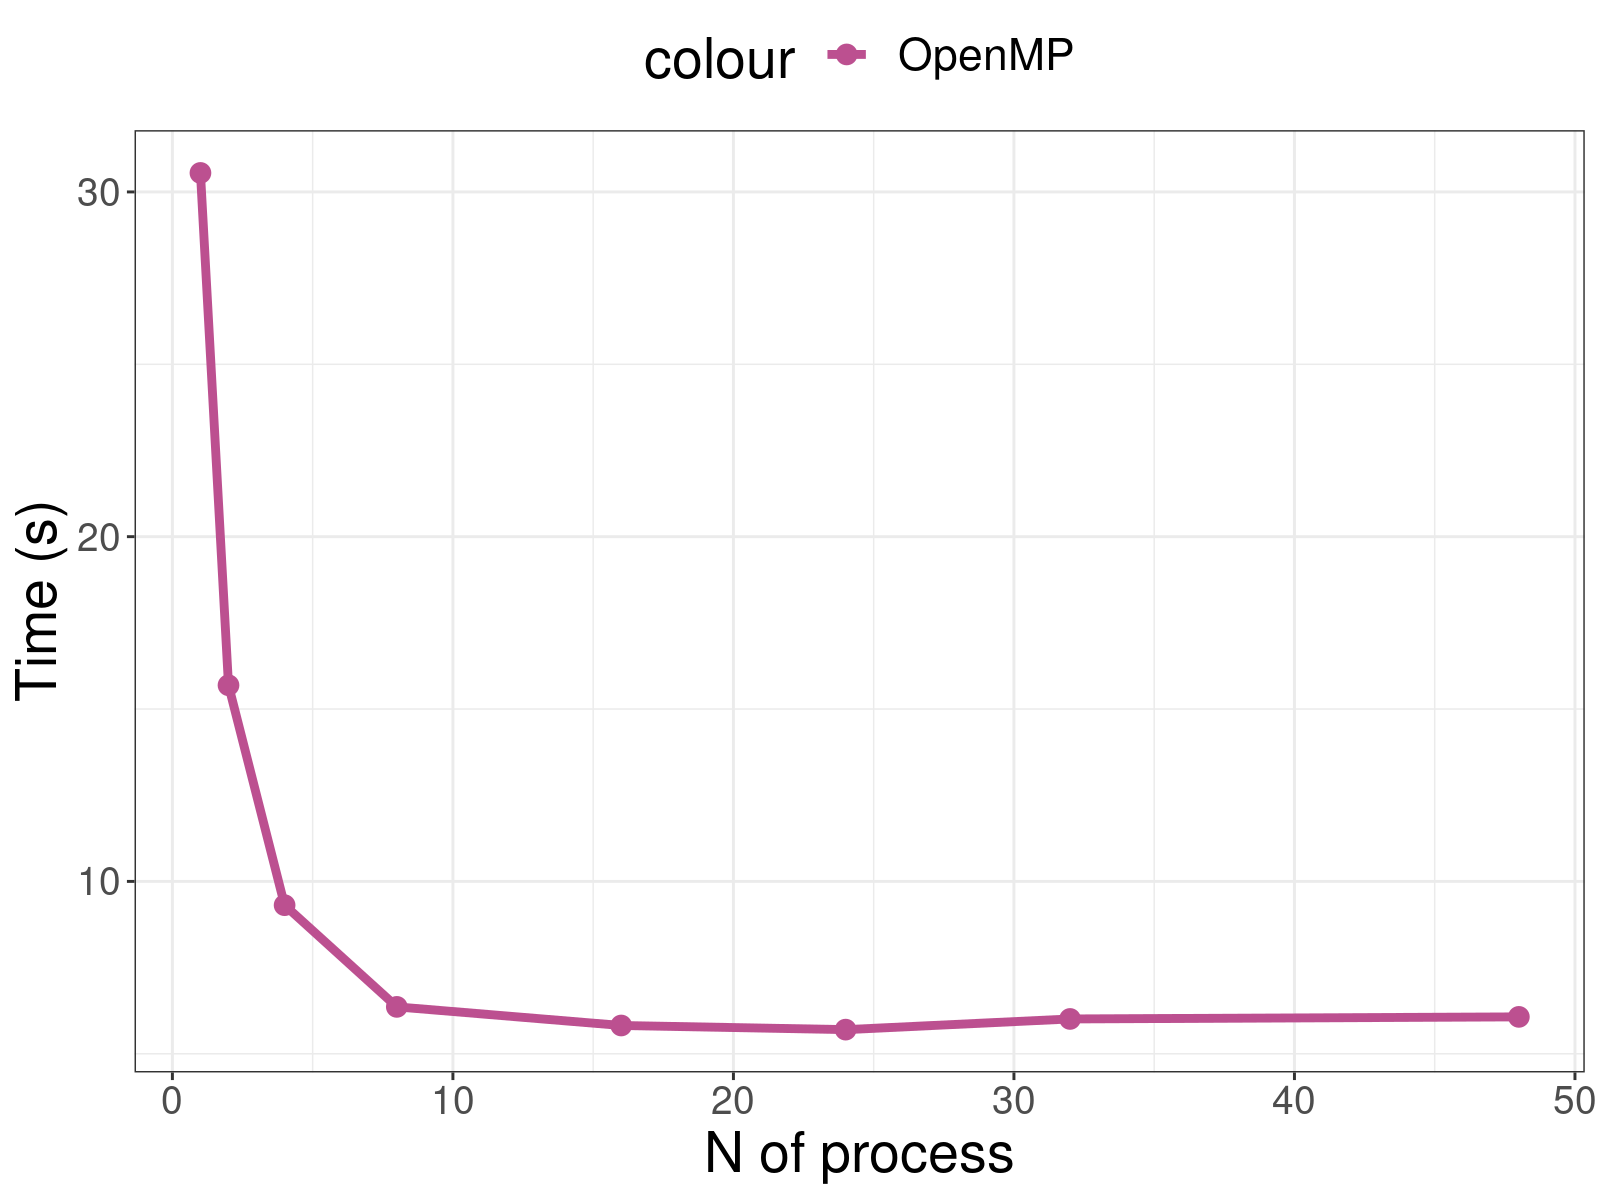
\includegraphics[width=8cm]{strong_OMP} }}
    \centering
    \subfloat[\centering Strong scalability OpenMPI]{{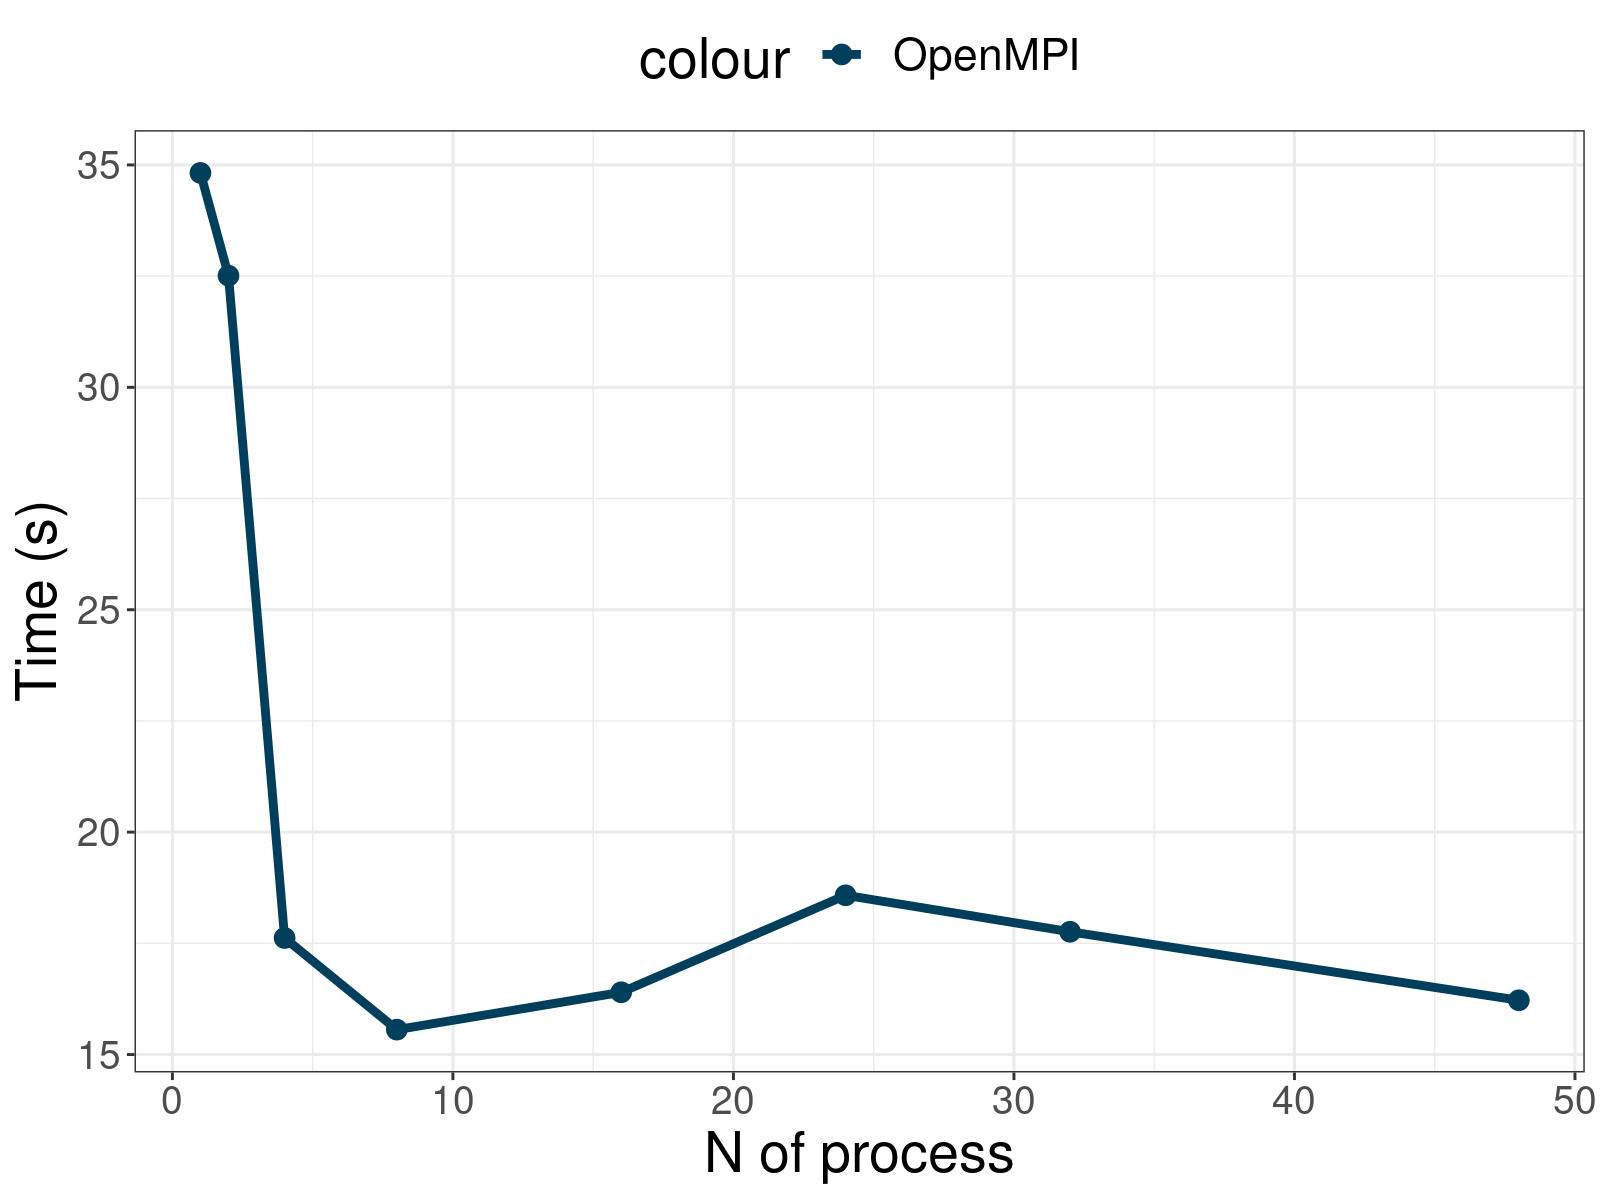
\includegraphics[width=8cm]{strong_MPI} }}
    \label{fig:example}%
\end{figure}
\subsection{Weak scalability}
In case of weak scalability, both the number of processes and the problem size are increased. The weak efficiency can be calculated by changing the problem size with each change of resources. The problem size was increased by a factor of 10 (starting from $10^{5}$), with each scale up in resources. Also in this case is possible to see how clearly the OpenMP implementation performe better with higher size. 
\begin{figure}[H]
    \centering
    \subfloat[\centering Weak scalability OpenMP \& OpenMPI]{{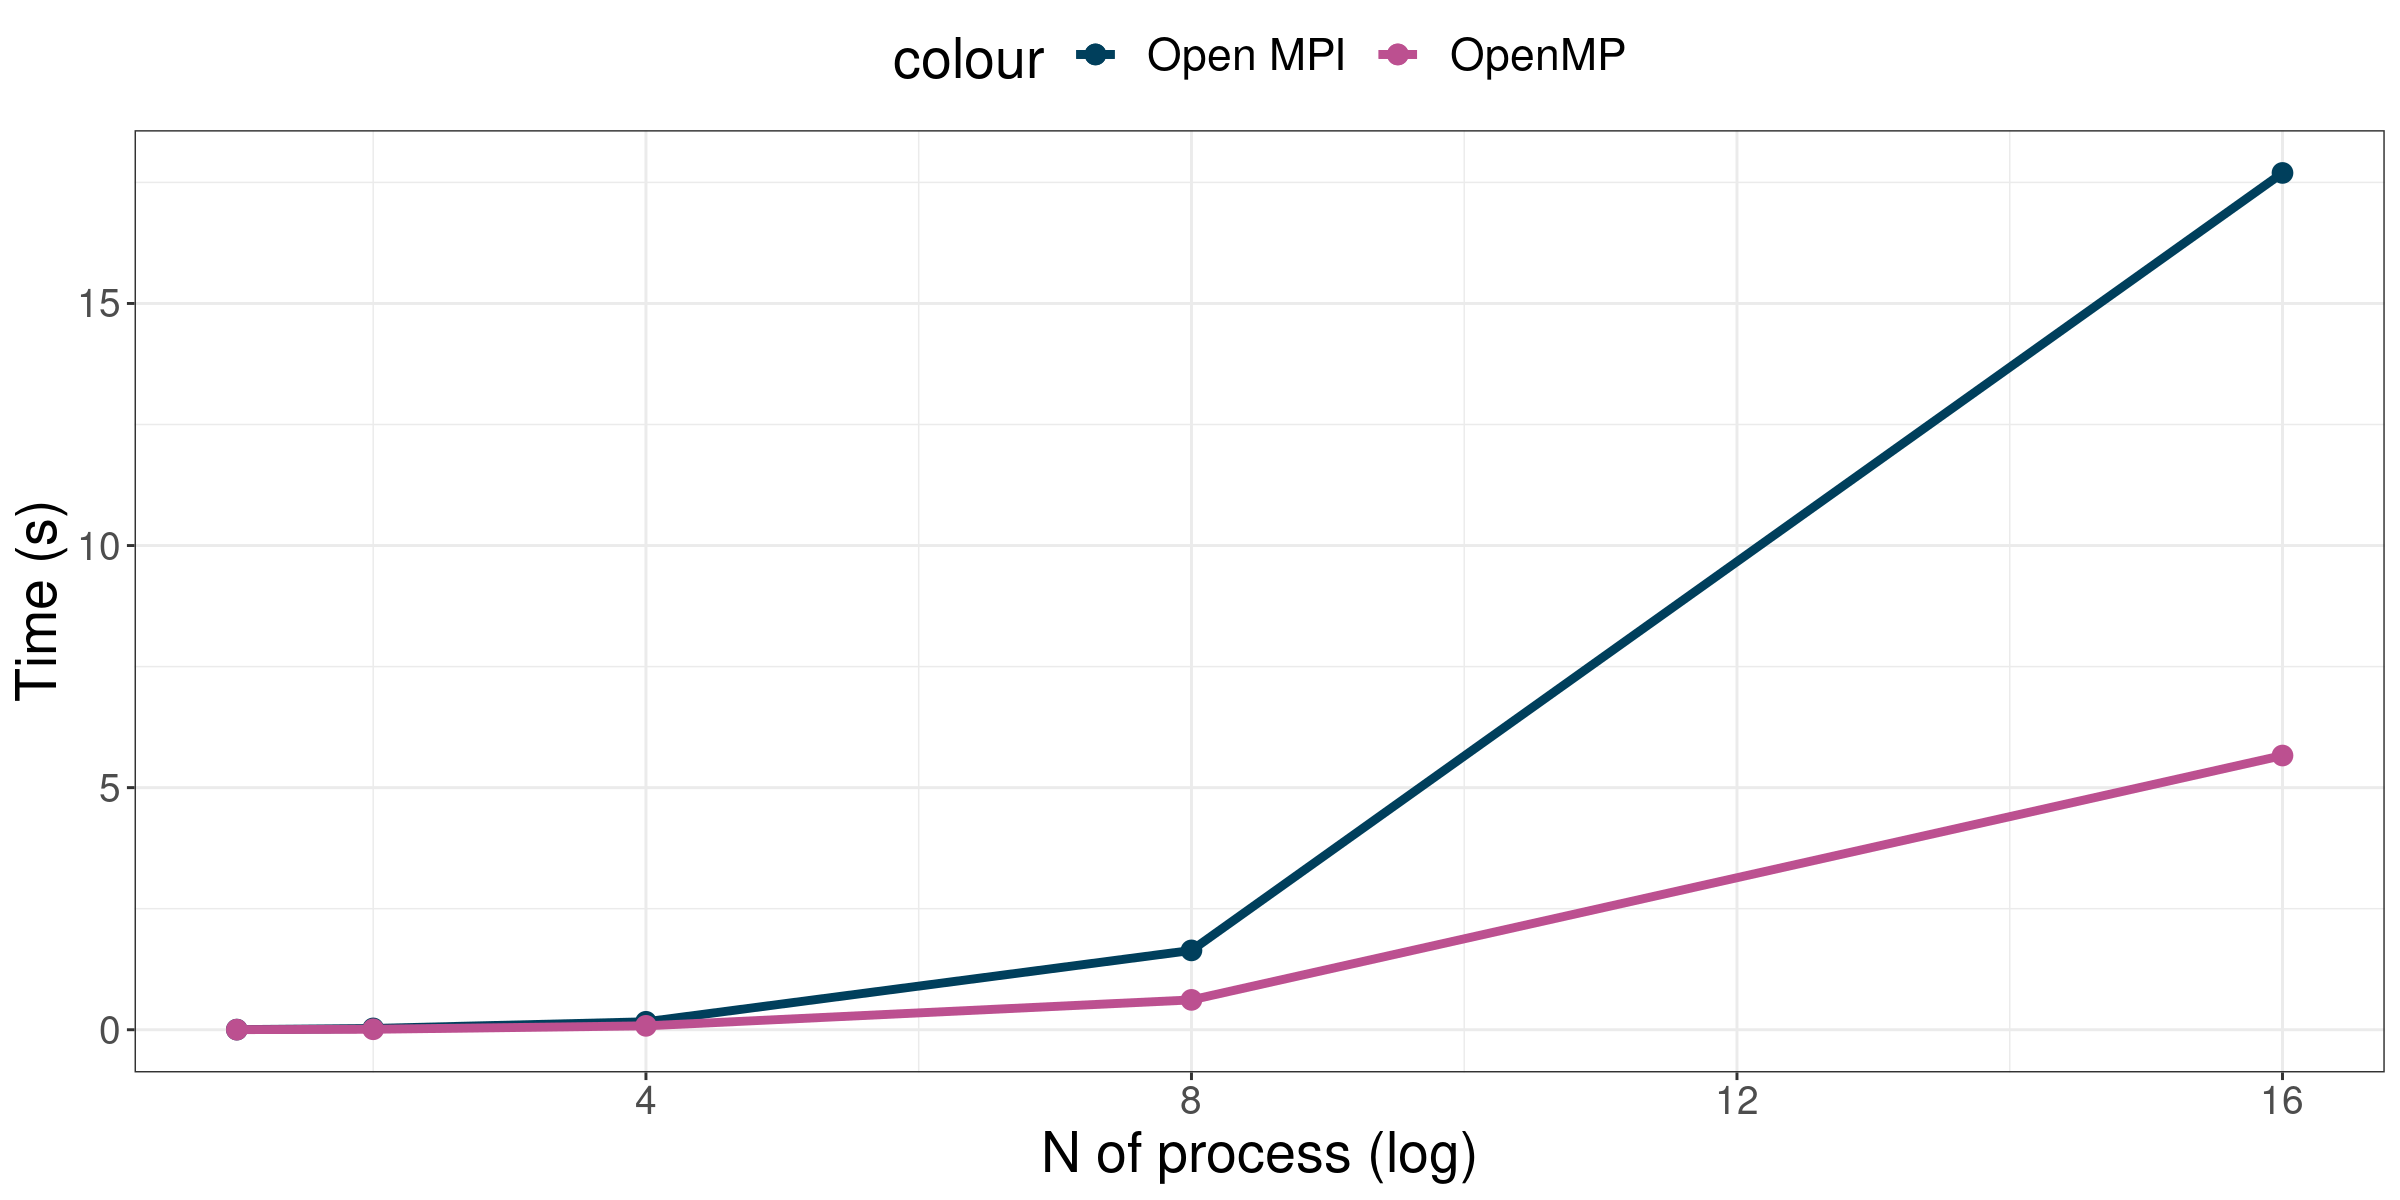
\includegraphics[width=15cm]{weak}}}
\end{figure}
\begin{figure}[H]
    \centering
    \subfloat[\centering Speedup OpenMP and OpenMPI]{{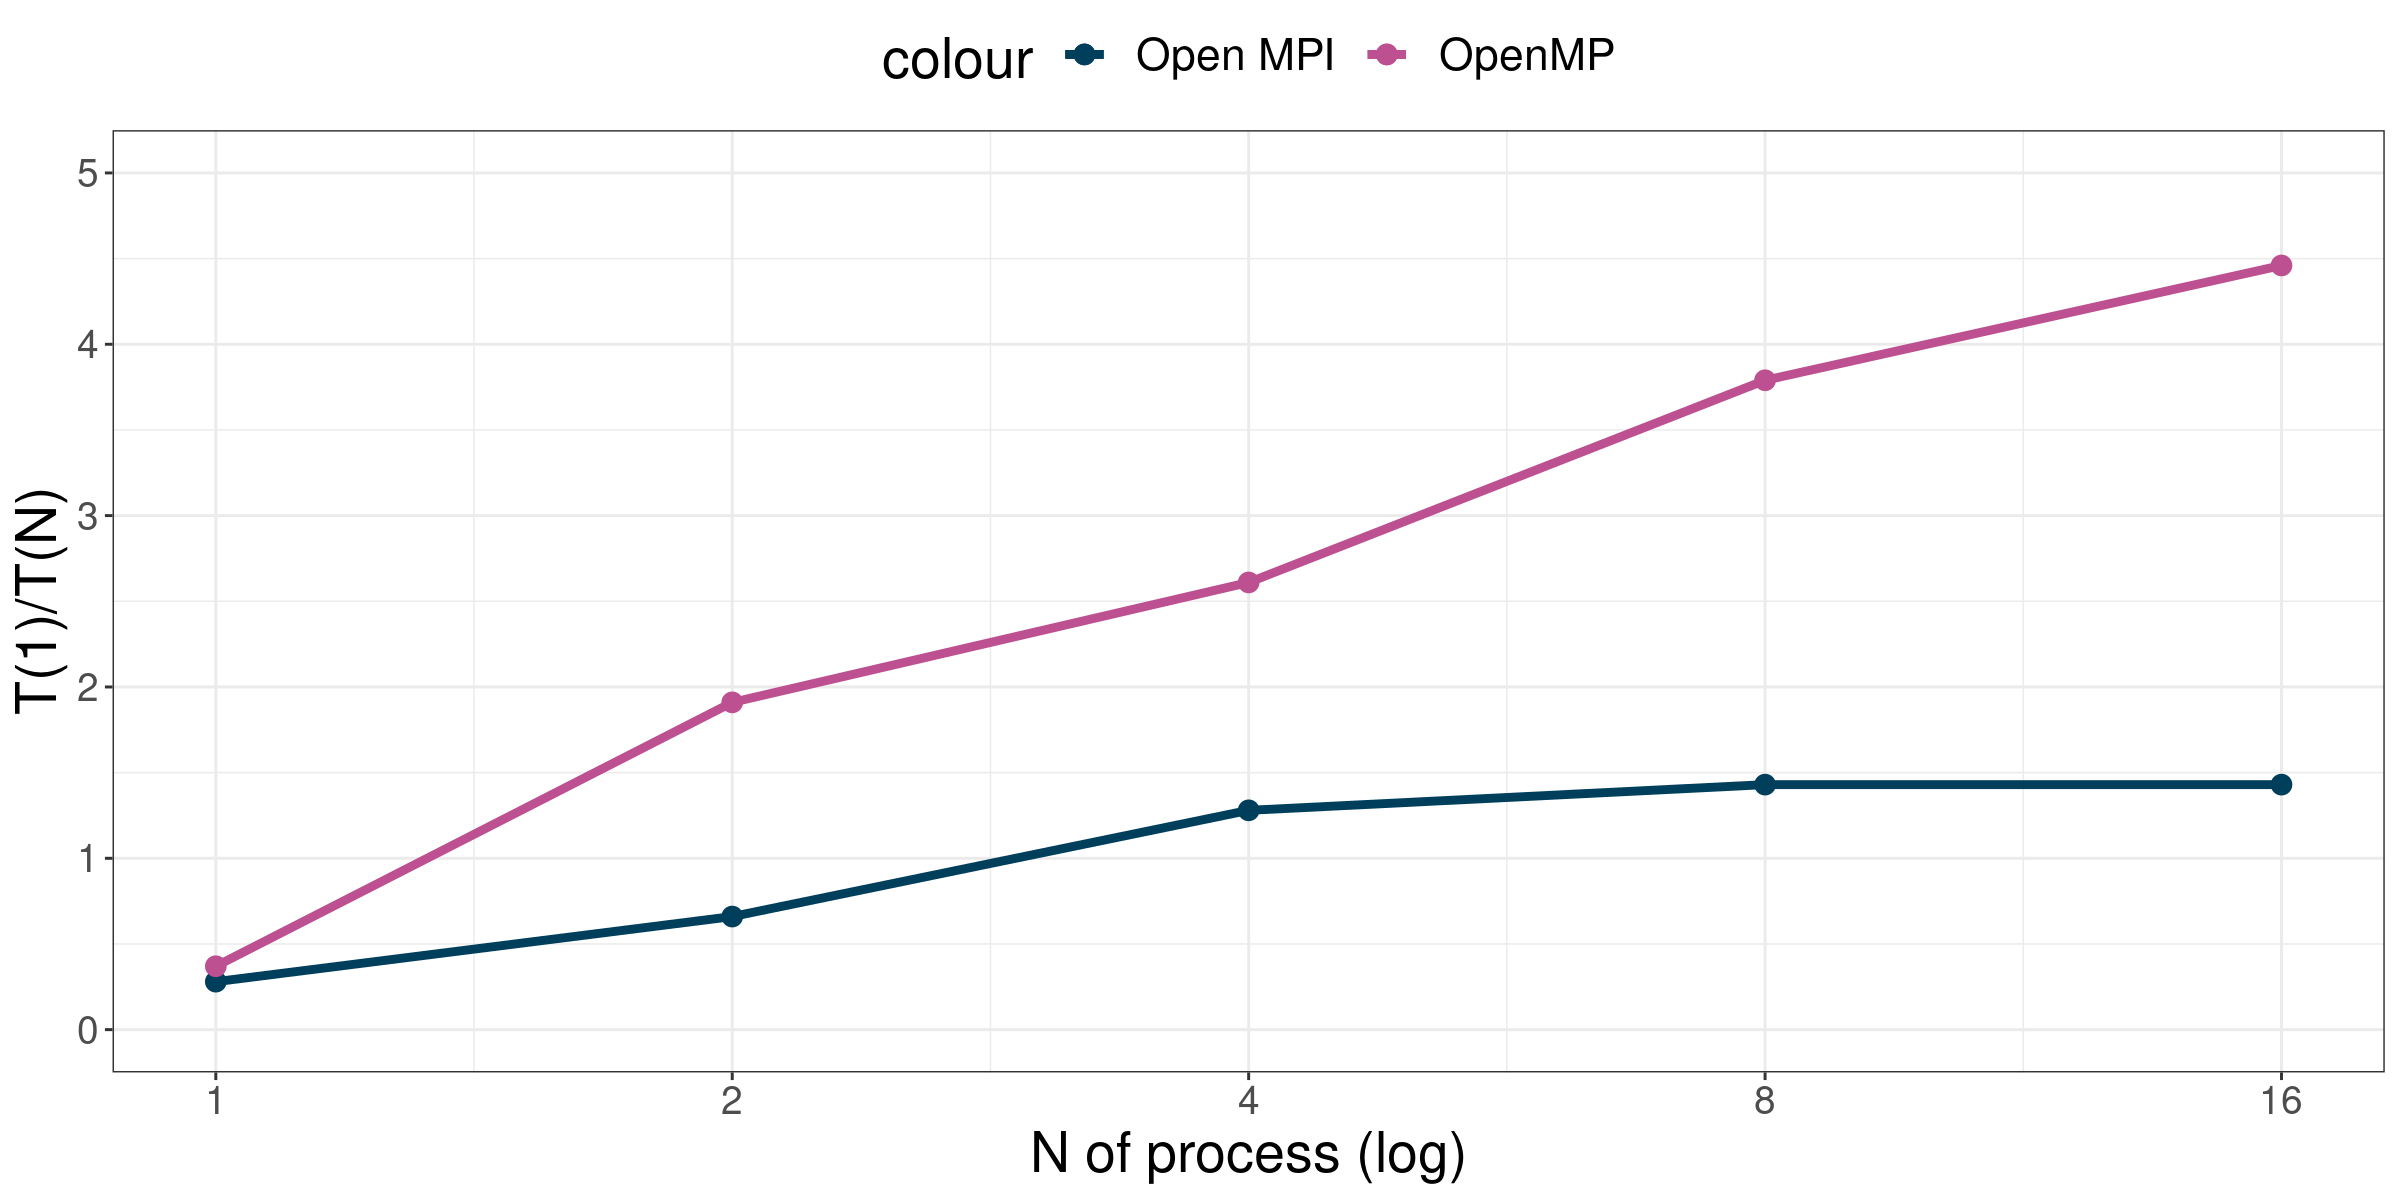
\includegraphics[width=15cm]{speedupWeak}}}
\end{figure}
\section{Conclusion}
From this work is possible to see how OpenMP performes well the work in the construction of the k-d tree. In the other hand clearly OpenMPI must be improved and a possible solution to this is by removing the entire serialization and deserialization part sending instead the entire sub-tree to the master process.
From the user point of view the final OpenMP solution has a better proportion between readability / performance. To improve the overall efficiency of the code a future implementation can be growing the k-d tree directly from the file taken in input without using $std::vector$ and to add some other functions like adding and deleting knodes. 
\end{document}
